\documentclass[11pt]{article}
%\usepackage{cite} % nicht kompatibel mit biblatex

\usepackage{hyperref}
%biblio
%\usepackage[style=alphabetic,citestyle=authoryear]{biblatex}
%\addbibresource{mybib.bib} %biblatex
%\usepackage{natbib}
\usepackage{url}
\usepackage{wrapfig}

%Math
\usepackage{amsmath}
\usepackage{amsfonts}
\usepackage{amssymb}
\usepackage{amsthm}
\usepackage{ulem}

%PageStyle
%\usepackage[ngerman]{babel} % deutsche Silbentrennung1
%\usepackage[utf8x]{inputenc} % nicht kompatibel mit biblatex
\usepackage{fancyhdr, graphicx}
\usepackage{subcaption}
\usepackage[scaled=0.92]{helvet}
\usepackage{enumitem}
\usepackage{parskip}
\usepackage[a4paper,top=2cm]{geometry}
\setlength{\textwidth}{17cm}
\setlength{\oddsidemargin}{-0.5cm}
\usepackage{lastpage} % for getting last page number
\renewcommand{\familydefault}{\sfdefault}
\usepackage{setspace}
\usepackage{acronym}


% Code listenings
\usepackage{color}
\usepackage{xcolor}
\usepackage{listings}
\usepackage[font=it]{caption}
\DeclareCaptionFont{white}{\color{white}}
\DeclareCaptionFormat{listing}{\colorbox{gray}{\parbox{\textwidth}{#1#2#3}}}
%\captionsetup[lstlisting]{format=listing,labelfont=white,textfont=white}
\lstset{
 language=Java,
 basicstyle=\footnotesize\ttfamily, % Standardschrift
 numbers=left,               % Ort der Zeilennummern
 numberstyle=\tiny,          % Stil der Zeilennummern
 stepnumber=5,              % Abstand zwischen den Zeilennummern
 numbersep=5pt,              % Abstand der Nummern zum Text
 tabsize=2,                  % Groesse von Tabs
 extendedchars=true,         %
 breaklines=true,            % Zeilen werden Umgebrochen
 frame=b,         
 %commentstyle=\itshape\color{LightLime}, Was isch das? O_o
 %keywordstyle=\bfseries\color{DarkPurple}, und das O_o
 basicstyle=\small,
 stringstyle=\color[RGB]{42,0,255}\ttfamily, % Farbe der String
 keywordstyle=\color[RGB]{127,0,85}\ttfamily, % Farbe der Keywords
 commentstyle=\color[RGB]{63,127,95}\ttfamily, % Farbe des Kommentars
 showspaces=false,           % Leerzeichen anzeigen ?
 showtabs=false,             % Tabs anzeigen ?
 xleftmargin=17pt,
 framexleftmargin=17pt,
 framexrightmargin=5pt,
 framexbottommargin=4pt,
 showstringspaces=false      % Leerzeichen in Strings anzeigen ?        
}

%Config
\fancypagestyle{firststyle}{ %Style of the first page
 \fancyhf{}
 \fancyheadoffset[L]{0.6cm}
 \lhead{
 
\includegraphics[scale=0.8]{./fhnw_logo.jpg}}
 \renewcommand{\headrulewidth}{0pt}
 \lfoot{Institute for Data Science,\linebreak www.fhnw.ch }
}

\fancypagestyle{documentstyle}{ %Style of the rest of the document
 \fancyhf{}
 \fancyheadoffset[L]{0.6cm}
\lhead{
 
\includegraphics[scale=0.8]{./fhnw_logo.jpg}}
 \renewcommand{\headrulewidth}{0pt}
 \lfoot{Forced Alignment with a Recurrent Neural Network}
 \rfoot{\thepage\ / \pageref{LastPage} }
}

\fancypagestyle{tableofcontent}{ %Style of the rest of the document
 \fancyhf{}
 \fancyheadoffset[L]{0.6cm}
\lhead{
 
\includegraphics[scale=0.8]{./fhnw_logo.jpg}}
 \renewcommand{\headrulewidth}{0pt}
 \cfoot{\thepage}
}

\fancypagestyle{abstract}{ %Style of the first page
 \fancyhf{}
 \fancyheadoffset[L]{0.6cm}
 \lhead{
 
\includegraphics[scale=0.8]{./fhnw_logo.jpg}}
 \renewcommand{\headrulewidth}{0pt}
 \cfoot{}
}


%Metadata
\numberwithin{equation}{section}

\begin{document}
\title{IP9}
\author{Daniel Tiefenauer}
\date{\today}
\maketitle

\newpage
\pagestyle{abstract}
\section*{Abstract}
tbd.

%TOC
\newpage
\pagestyle{tableofcontent}
\pagenumbering{Roman}
\tableofcontents  	
\newpage

\pagestyle{documentstyle}
\setcounter{page}{1}
\pagenumbering{arabic}

\section{Introduction}\label{intro}
This report documents the progress of the project \textit{Speech-To-Text Engine for Forced Alignment}, my master thesis at \ac{FHNW} (referred to as \textit{IP9}). Some preliminary work has been done in a previous project (referred to as \textit{IP8}). The overall goal, project situation and some background information are described in detail in the project report for IP8 and shall not be repeated here. A quick recap of the relevant terms and aspects is given as far as they are relevant for the understanding of this document.

\subsection{Scope and overall goal}
\textit{ReadyLingua} is a Switzerland based company that develops tools and produces content for language learning. Some of this content consists of audio/video data with an accompanying transcript. The overall goal is to enrich the textual data with temporal information, so that for each part of the transcript the corresponding point in the audio/video data can be found. This process is called \textit{ac{fa}}. An \textit{InnoSuisse} project was started in 2018 to research how this could be achieved. The \textit{InnoSuisse} project foresees three different approaches, one of which is pursued in this project.

\subsection{Chosen approach and previous work}
The approach chosen for this project is based on speech pauses, which can be detected using \textit{\ac{VAD}}. The utterances in between are transcribed using \textit{\ac{ASR}}, for which a \textit{\ac{RNN}} is used. The resulting partial transcripts contain the desired temporal information and can be matched up with the full transcript by means of \ac{LSA}.

All theses parts were treated as individual stages of a pipeline:

\begin{itemize}
	\item \textbf{\ac{VAD}}: the audio was split into non-silent parts
	\item \textbf{\ac{ASR}}: each part was transcribed resulting in a partial transcript, which can contain transcription errors
	\item \textbf{\ac{LSA}}: each partial transcript was localized within the original transcript	
\end{itemize}

Since the quality of the \ac{ASR} stage has an imminent impact on the subsequent \ac{LSA} stage, the quality of the alignments depends heavily on the quality of the partial transcripts. This makes the \ac{ASR} stage the crucial stage of the pipeline. However, \ac{ASR} is highly prone to external influences like background noise, properties of the speaker (gender, speaking rate, pitch, loudness). Apart from that, language is inherently abiguous (e.g. accents), inconsistent (e.g. linguistic subtleties like homonyms or homophones) and messy (stuttering, unwanted repetitions, mispronunciation).

\subsubsection{Previous results and problems}
For the \ac{VAD} stage, an implementation\footnote{\url{https://github.com/wiseman/py-webrtcvad}} of \textit{WebRTC}\footnote{\url{https://webrtc.org/}} was used. This implementation which has proved to be capable of detecting utterances with very high accuracy within reasonable time. For the \ac{LSA} stage a combination of the Smith-Waterman algorithm and the Levenshtein distance was used. This combination included tunable parameters and proved to be able to be able to localize partial transcript within the full transcript pretty well, provided the similarity between actual and predicted text was high enough. 

For the \ac{ASR} stage on the other hand, no \ac{RNN} could be trained that was capable of transcribing the audio segments with a quality that was high enough for the \ac{LSA} stage. The main problems were the lack of readily available training data in high quality, very long training times and therefore very long feedback cycles. Because the \ac{ASR} stage is at the heart of the pipeline, the self-trained model was replaced by \ac{GCS}\footnote{\url{https://cloud.google.com/speech-to-text/}}, which was embedded into the pipeline over an API. This step however made the pipeline dependent on a commercial product, whose inner workings remain unknown and who cannot be tuned to the project's needs. Furthermore, although the quality of the transcriptions produced by \ac{GCS} is very good, it might be an overkill for the purpose of this project and the API calls are subject to charges.

The IP8 project proposed the use of \textit{DeepSpeech} for the \ac{ASR} stage, which uses \ac{CTC} \parencite{ctc_paper} as its cost function. Some experiments were made to find out what features can be used to train a \ac{RNN} for the \ac{ASR} stage. The features considered were raw power-spectrograms (as stipulated by the \textit{DeepSpeech} paper), Mel-Spectrograms and \ac{MFCC}. It was found that training on \ac{MFCC} features would probably require the least amount of training data because. An \ac{RNN} using a simplified version of the \textit{DeepSpeech} architecture was trained on data from the \textit{LibriSpeech} project (containing only English samples). However, developing a fully-fletched ASR system is extremely time-consuming and could not be done within the project time. For that reason a state-of-the-art \textit{\ac{STT}} engine (\textit{Google Cloud Speech}) was embedded in the pipeline as the \ac{ASR} stage. Using this engine, the pipeline was able to produce very good (although not perfect) transcripts for the individual utterances. Therefore the chosen approach was validated and the pipeline could shown to be generally functional.

\subsection{Goal of this project}

In this project, the chosen pipelined approach shall further be refined. Because the \ac{VAD} and the \ac{LSA} stage already work pretty well, the focus in this project lies on the \ac{ASR} stage. Because the pipeline should become language-agnostic and self-contained, a \ac{RNN} must be trained that can be used in this stage in the pipeline. Such a \ac{RNN} could be a simplified variant of the \textit{DeepSpeech} model. The idea behind this are the following two points:

\begin{itemize}
	\item A simpler model will not be able to produce transcripts with the same quality as complex models like \textit{DeepSpeech} or \ac{GCS}. But since the superordinated goal of this project is \ac{FA} and not Speech Recognition, this may not be required in the first place. The \ac{RNN} only needs to be \textit{good enough} for the downstream \ac{LSA} stage
	\item On the other hand, a simpler model will probably need less training data to learn. This might open up new possibilities to align audio and text in other languages, for which there is not a third-party solution yet, such as Swiss German.
\end{itemize}

The goal of this project is therefore to make statements as to under what conditions the \ac{ASR} stage can be implemented. For this, various combinations of network or data properties are explored as well as varying amounts of training data. Concretely, the following questions shall be answered:

\begin{itemize}
	\item \textbf{How does the quality of the simplified \textit{DeepSpeech}-\ac{RNN} change with increasing training data?} By plotting the learning curve we should be able to see whether the RNN is able to learn something useful at all and also get some intuition about how much training data is needed to get reasonably accurate partial transcripts.
	\item \textbf{How does the quality of the partial transcripts change when using synthesized training data?} Neural Network usually require large amounts of training data and often improve with increasing size of the training set. However, labelled training data is usually scarce and/or expensive to acquire. For the purpose of Forced Alignment however, synthesized training data can be easily obtained by adding some distortion to the original signal (reverb, change of pitch, change of tempo).
	\item \textbf{How does the quality of the partial transcript change when integrating a \ac{LM}?} \ac{STT}-engines traditionally use a \ac{LM} that models the probabilities of characters, words or sentences. A \ac{LM} can help producing valid transcripts by mapping transcripts (that may sound similar to what was actually said) to orthographically correct sentences.
	\item \textbf{How can we assess the quality of the alignments?} This should give us some insight about how the quality of the alignment changes with varying capability of the \ac{STT}-engine and what quality of transcripts is required.
\end{itemize}

Answering above questions should help estimating the effort to create a generic pipeline. \footnote{Because \ac{ASR} is highly dependent on the language that should be recognized, a different \ac{STT} system has to be trained for each language.}


\newpage

\section{Training an \ac{RNN} for \ac{ASR}}\label{ds}
As stated above, this project does not aim at training a state of the art \ac{STT} engine. Because the \ac{SW} algorithm used for local alignment is tolerant to a certain amount of errors in the transcripts, the \ac{RNN} need only be \textit{good enough} for the task at hand (\ac{FA}). If such a network can be trained under the given circumstances it could be used in the \ac{ASR} stage of the pipeline. The pipeline would then become become self-contained and would not ne dependent on a commercial solution that cannot eb tuned and whose inner workings are unknown. Furthermore such a \ac{RNN} would open up to recognizing languages for which there is not a third-party solution yet, such as Swiss German.

\subsection{Exploiting the \textit{DeepSpeech} model}

A \ac{NN} that had quite an impact on \ac{ASR} was \textit{DeepSpeech} \cite{deepspeech} which reached recognition rates near-par to human performance, despite using a comparably simpler than traditional speech systems. Because the relation between audio signal and text was learned \ac{E2E} the network was also pretty robust to distortions like background noise or speaker variation. An open source implementation of a DeepSpeech model is available from Mozilla \footnote{\url{https://github.com/mozilla/DeepSpeech}}. Since this implementation uses a \ac{LM}, the quality of the model is measured as the percentage of misspelled or wrong words (called \ac{WER}) or as the edit distance (also called Levenshtein distance or \ac{LER}). A pre-trained model for inference of English transcript can be downloaded, which achieves a \ac{WER} of just 6.5\%, which is close to what a human is able to recognize \cite{mozillajourney}.

A model could be trained by providing training-, validation- and test-data for an arbitrary language (e.g. from the \textit{ReadyLingua} corpus). However, this is not the preferred procedure for this project for various reasons:

\begin{enumerate}
	\item The \textit{DeepSpeech} implementation was designed for \ac{ASR}. In such settings a low \ac{WER} is desirable. But this is not the main focus for this project. As a result, the architecture of the Mozilla implementation might be overly complicated for this project, although it might make sense for pure \ac{ASR} tasks. 
	\item The problem with above point is that more complex models usually require more training data. However, as for any neural network, the limiting factor for training a \ac{RNN} is often the lack of enough high quality training data. This becomes especially important when recordings in a minority language should be aligned. 
	\item The implementation requires an (optional) \ac{LM}, which is tightly integrated with the training process which might not be available for the target languages.
\end{enumerate}

For these reasons, the \ac{RNN} architecture of the \textit{DeepSpeech} model was used as a basis for a simplified version, which should (hopefully) require less training data in order to converge and still produce partial transcriptions that can be locally aligned.

\subsection{A simpler \textit{DeepSpeech} model}

An implementation of the \ac{RNN} used for \ac{STT} in the previous IP8 project was done in Python using Keras\footnote{\url{https://keras.io}}. The following simplifications and alterations were made:

\begin{itemize}
	\item No \ac{LM} 
	\item No convolution in first layer
	\item LSTM instead of SimpleRNN
\end{itemize}

Figure tbd. shows the architecture proposed in the \textit{DeepSpeech} compared to the simplified version used in this project / with the changes made for this project (eines von beidem verwenden).

tbd: Hier Bild Architektur einfügen

However, despite training on the \textit{LibriSpeech} corpus, this network did not seem converge. Furthermore, performance was a big issue, although the \ac{RNN} used a simpler architecture and no computational power was needed to query a \ac{LM}. Training on aligned speech segments from the \textit{LibriSpeech} corpus was not possible within project time because it would have taken approximately two months when using a single ac{GPU}. However, this duration is at least consistent with the experience made by the Machine Learning team at Mozilla Research, which used a cluster of 16 \acsp{GPU} that required about a week \cite{mozillajourney} to train a variant \footnote{the variant used \ac{MFCC} as features whereas the original paper proposed raw spectrograms} of the \ac{RNN} originally proposed in \cite{ctc_paper}.

In this project some experimentation was done to make the model converge:

\begin{itemize}
	\item increased number of MFCC features from 13 to 26, because this is the value used in the \textit{DeepSpeech} model
	\item tried out different optimizers. Surprisingly, SGD seemed to work better than Adam
	\item switched back to a Simple RNN instead of LSTM
	\item include a language model
\end{itemize}

\section{Including a \ac{LM}}

Although \ac{CTC} is the cost that is optimized during training, the main metrics to evaluate an \ac{ASR} system are usually \ac{WER} and \ac{LER}. The \ac{LER} is defined as the mean normalized edit distance ($ed(a, b)$ i.e. the number of insertions, deletions and changes required to produce string $b$ from string $a$) between a an inferred transcription (\textit{prediction}) and the actual transcription (\textit{ground truth} or \textit{label}). It operates on character level and is sometimes also referred to as \textit{Levensthein Distance}. The \ac{WER} builds upon the \ac{LER} but operates on word level, i.e. it represents the number of words in a inferred transcription, that need to be inserted, deleted or changed in order to arrive at the ground truth.

If a single evaluation metric is required, the \ac{WER} is often the better choice because it is more related to the way humans would assess the quality of a transcription: A transcription which might sound correct when read out loud but is full of spelling mistakes is not a good transcription. A \ac{LM} can help inferring orthographically correct words from sequences of characters detected by \ac{CTC} and hence decrease the \ac{WER}. Therefore, by using a \ac{LM} the quality of transcriptions improves perceivably, as the following example shows:

\begin{table}[!htbp]
	\centering
	\begin{tabular}{|l|l|r|}
		\hline
		\thead{transcript} & \thead{value} & \thead{\ac{LER}} \\
		\hline
		actual transcript & \code{and i put the vice president in charge of mission control} & $1.00$ \\ 
		\hline
		inference without LM & \code{ii put he bice president in charge of mission control} & $0.11$ \\ 
		\hline
		inference with LM & \code{i put the vice president in charge of mission control} & $0.08$ \\
		\hline
	\end{tabular}
	\caption{examples of infered transcripts with pre-trained DeepSpeech model with and without \ac{LM}\\(sample \code{20161203potusweeklyaddress} from the ReadyLingua corpus}
\end{table}

tbd: Hier kurz LM zusammenfassen (n-Gram erklären)

The Mozilla implementation includes an n-Gram \ac{LM} using \textit{KenLM}. The \ac{LM} is queried while decoding the numeric matrices produced by \ac{CTC} using \textit{Beam Search} or \textit{Best-Path} decoding. It uses a \textit{trie} and precompiled custom implementations in C of \textit{TensorFlow}-operations to maximize performance and dedicated weights for the influence the number of valid words and the \ac{LM} itself on the inferred transcription. It is therefore deeply baked in with the decoding process.

A simpler variant that is used in this project is to infer the transcriptions first with \textit{Beam Search} or \textit{Best-Path} decoding using the standard tools provided by Keras. The inferred transcriptions are then post-processed by running it through some sort of spell-checking, which is done as follows:

\begin{itemize}
	\item split the sentence into words 
	\item for each word $w_i$ in the sentence check the spelling by generating the set $C_i$ of possible corrections by looking it up in $V$, the vocabulary of the \ac{LM}, as follows:
	\begin{itemize}
		\item if $w_i \in V$ its spelling is already correct and $w_i$ is kept as the only possible correction, i.e.
		\begin{equation*}
			C_i = C_j^0 = \{ w_i \}
		\end{equation*}
		\item if $w_i \not\in V$ generate $C_i^1$ as the set of all possible words $w_i^1$ with $ed(w_i, w_i^1) = 1$. This is the combined set of all possible words with one character inserted, deleted or replaced. Keep the words from this combined set that appear in $V$, i.e.
		\begin{equation*}
			C_i = C_i^1 = \left \{ w_i^1 \mid (w_i, w_i^1) = 1 \land w_i^1 \in V \right \}
		\end{equation*}
		\item if $C_i^1 = \emptyset$ generate $C_i^2$ as the set of all possible words $w_i^2$ with $ed(w_i, w_i^2) = 2$. $C_i^2$ can be recursively calculated from $C_i^1$. Again only keep the words that appear in $V$, i.e.
		\begin{equation*}
			C_i = C_i^2 = \left \{ w_i^2 \mid ed(w_i, w_i^2) = 2 \land w_i^2 \in V) \right \}
		\end{equation*}
		\item if $C_i^2 = \emptyset$ keep $w_i$ as the only word, accepting that it might be either misspelled, a wrong word, gibberish or simply has never been seen by the \ac{LM}, i.e.
		\begin{equation*}
			C_i = C_i{>2} = \left \{ w_i  \right \}
		\end{equation*}
	\end{itemize}
	\item for each possible spelling in $C_i$ build the set $P$ of all possible 2-grams with the possible spellings in the next word as the cartesian product of all words, i.e.
	\begin{flalign*}
&	P = \{ (w_j, w_{j+1} | w_j \in C_j \land w_{j+1} \in C_{j+1} \}{,} && C_j \in \{C_i^0, C_i^1, C_i^2, C_i^{>2} \}
	\end{flalign*}
	\item score each 2-gram calculating the log-based probability using a pre-trained 2-gram-\ac{LM}
\end{itemize}

\section{Plotting a learning curve}

The total length of all transcribed speech segments in the \textit{LibriSpeech} corpus is roughly 47 days (1141 hours). Training on all these samples was not feasible within project time . However, we can get an estimation of the expected learning progress by plotting a \textit{learning curve}. This was done using transcribed audio segments from the \textit{LibriSpeech} corpus. Training was done on exponentially increasing amounts of training data (1, 10, 100 and 1000 minutes of transcribed audio).

\begin{figure}
	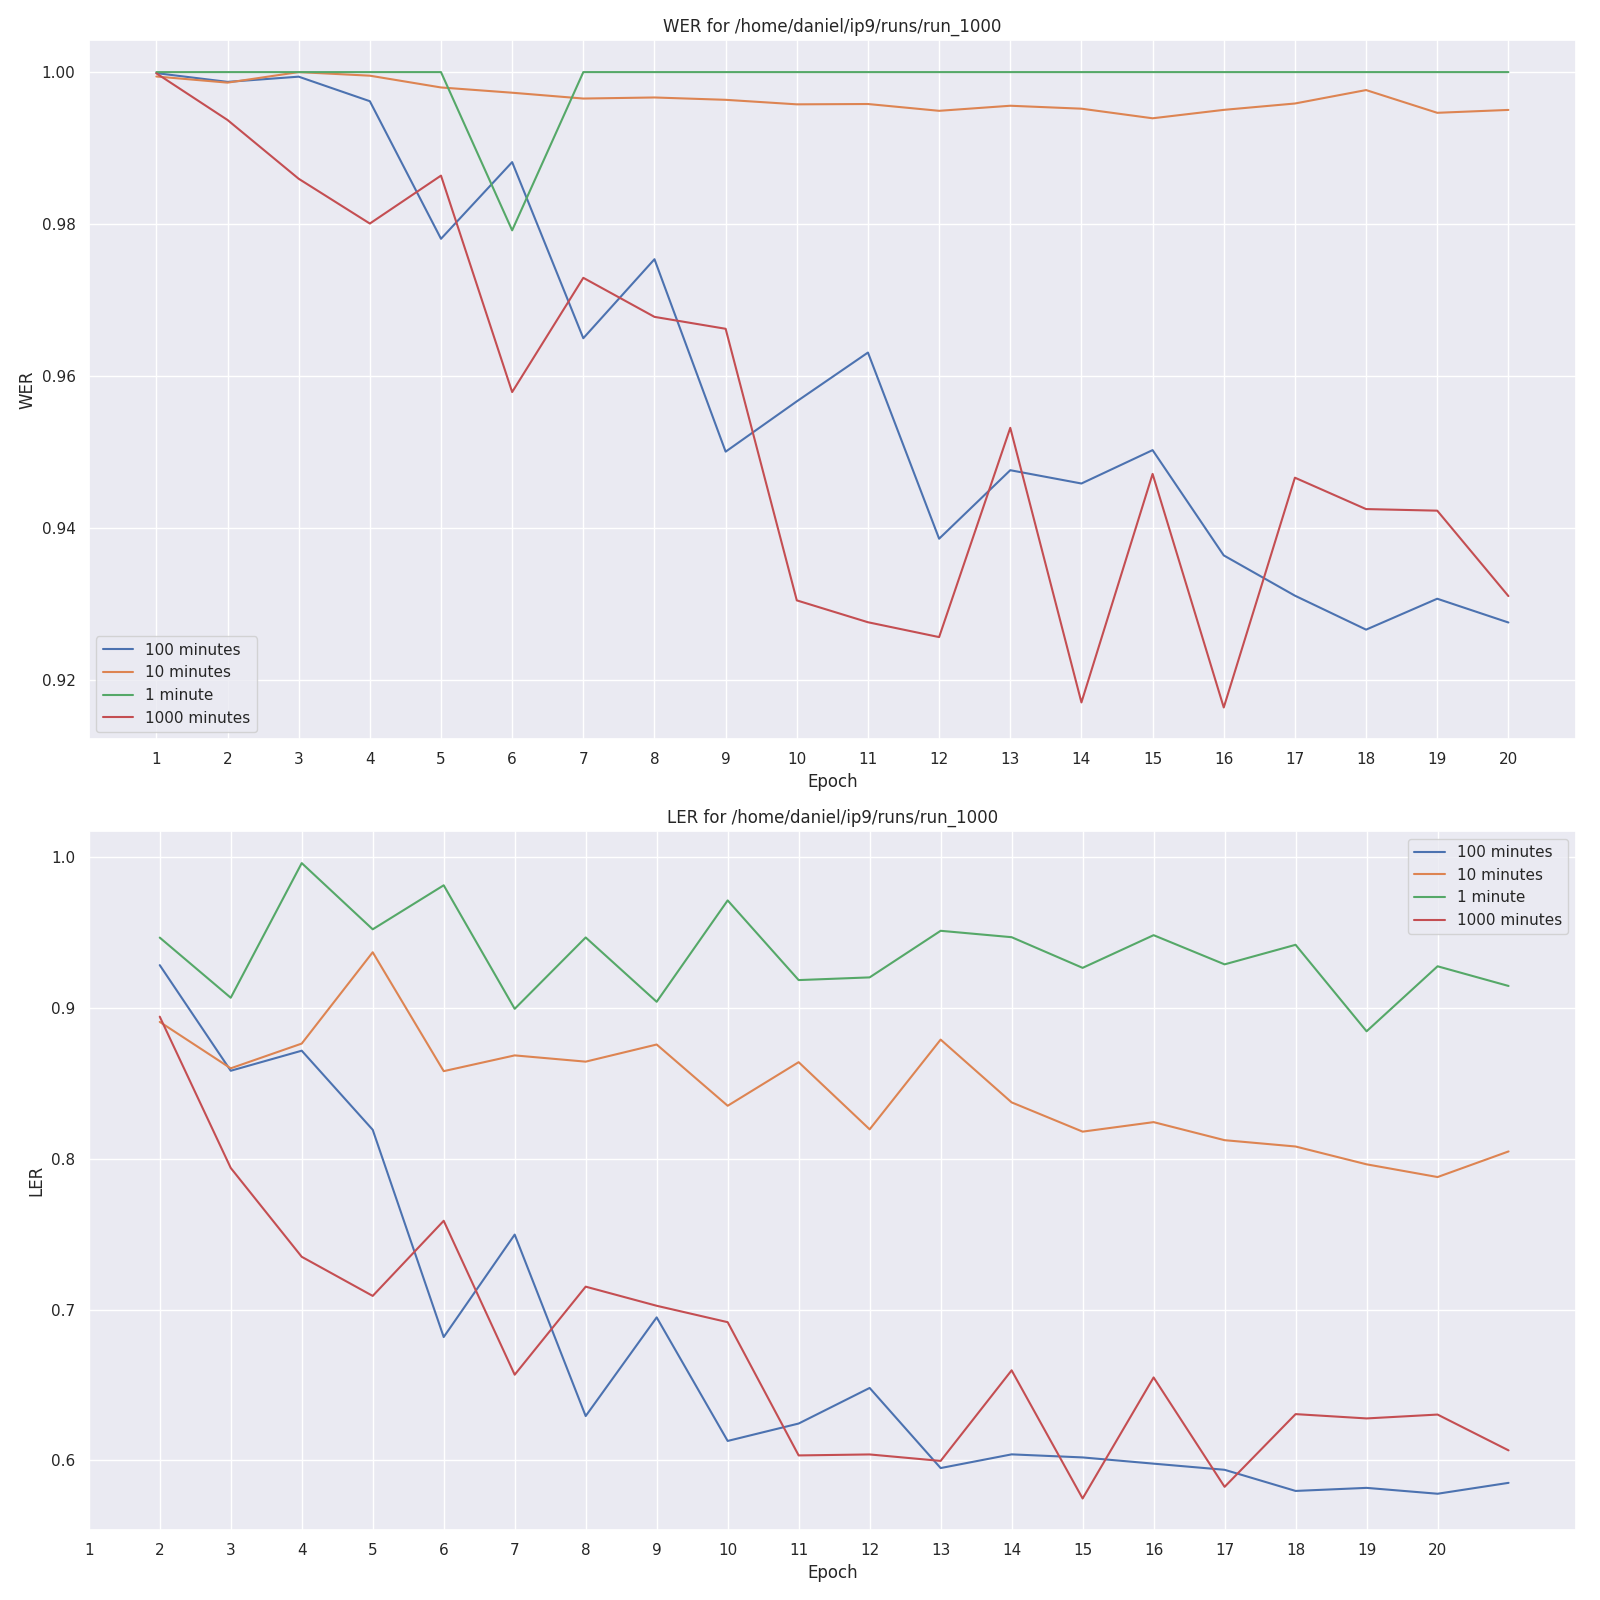
\includegraphics[width=\linewidth]{./img/learning_curve_lm_beamsearch.png}
	\caption{Learning curve for training on 1/10/100/1000 minutes of transcribed audio from \textit{ReadyLingua} using a 2-gram \ac{LM} and Beam-Search decoding}
\end{figure}

% To do:
% - train on LibriSpeech data
% - train using Best-Path
% - train using no LM
% - Reset calculation of WER/LER to original implementation
\newpage

%\bibliographystyle{plain}
\bibliographystyle{unsrt}
\bibliography{mybib}{}
%\printbibliography %biblatex command
\newpage

\listoffigures
\listoftables

\newpage
\section*{Acronyms used in this document}

\begin{acronym}[Bash]
	\acro{ASR}[ASR]{Automatic Speech Recognition}
	\acro{CTC}[CTC]{Connectionist Temporal Classification}
	\acro{DS}{Deep Speech}
	\acro{E2E}{end-to-end}
	\acro{FA}[FA]{Forced Alignment}
	\acro{FHNW}[FHNW]{University of Applied Sciences}
	\acro{GPU}[GPU]{Graphics Processing Unit}
	\acro{GRU}{Gated Recurrent Unit}
	\acro{LER}[LER]{Label Error Rate}
	\acro{LM}[LM]{Language Model}
	\acro{LSTM}{Long Short Term Memory}
	\acro{LSA}[LSA]{Local Sequence Alignment}
	\acro{MFCC}[MFCC]{Mel-Frequency Cepstral Coefficients}
	\acro{NN}{Neural Network}
	\acro{RNN}[RNN]{Recurrent Neural Network}
	\acro{SGD}{Stochastic Gradient Descent}
	\acro{STT}[STT]{Speech-To-Text}
	\acro{OOV}{Out Of Vocabulary}
	\acro{SRILM}{the SRI Language Modelling Toolkit}
	\acro{SW}{Smith Waterman}
	\acro{VAD}[VAD]{Voice Activity Detection}
	\acro{WER}[WER]{Word Error Rate}
\end{acronym}
\newpage
\section{Ehrlichkeitserklärung}
Hiermit erkläre ich, dass ich die vorliegende schriftliche Arbeit
selbstständig und nur unter Zuhilfenahme der in den Verzeichnissen oder
in den Anmerkungen genannten Quellen angefertigt habe. Ich versichere
zudem, diese Arbeit nicht bereits anderweitig als Leistungsnachweis
verwendet zu haben. Eine Überprüfung der Arbeit auf Plagiate unter
Einsatz entsprechender Software darf vorgenommen werden.\\
Würenlingen, \today\\[4\baselineskip]
Daniel Tiefenauer

\end{document}